\documentclass[pfc]{imetex}
\usepackage[table]{xcolor}
\usepackage{graphicx}

%% Capa
\firstAuthor{Victor Villas Bôas Chaves}
\secondAuthor{Lucas Sousa Meireles}
\thirdAuthor{Cláudio Cavalcante Bomfim}

\title{Identification by Keystroke Dynamics}
\date{Dezembro 2017}

%% Folha de Rosto
\preamble{Relatório Final do Programa Institucional de Bolsas de
Iniciação em Desenvolvimento Tecnológico e Inovação do
CNPq / Instituto Militar de Engenharia.}
\advisor{Prof. Ronaldo Goldschmidt}

%% Resumo
\vernacularAbstract{
Nosso resumão
}
\vernacularKeywords{dinâmica da digitação, reconhecimento de usuário}
\vehicularAbstract{
Our big abstract
}
\vehicularKeywords{our keywords}

%% Referências
\references{bibliografia}

\begin{document}

\chapter{Introdução}

\section{Contexto e Motivação}
Sistemas de Segurança da Informação modernos não se baseiam e um único método de autenticação, mas incrementalmente adicionam mecanismos com múltiplos fatores. Quanto mais e melhores fatores, maior a certeza da identidade ser autenticada corretamente.

Dentre as alternativas mais promissoras estão os fatores biométricos, valorizados por sua natureza individual e difícil falsificação. Os fatores biométricos frequentemente mencionados são os fisiológicos, mas seu emprego traz diversos fatores complicantes como a necessidade de amostragem prévia e diminuição da usabilidade do sistema. Uma alternativa é o uso de fatores biométricos de comportamento, como padrões comportamentais expressos naturalmente pelo usuário.

As vantagens dos fatores comportamentais incluem a possibilidade de amostragem silenciosa, maior variabilidade do grau de confiança e a transparência do mecanismo para o usuário. Em particular, sistemas providos pela \textit{Web} em geral possuem uma uniformidade de interface que permite a coleta de vários padrões comportamentais durante todo o uso do sistema.

Alguns exemplos de comportamentos de interesse coletáveis incluem padrões de digitação, cliques de \textit{mouse} ou áreas do sistema e recursos acessadas pelo usuário. A pesquisa sobre como utilizar fatores dessa natureza pode impulsionar sistemas mais seguros e menos impactantes na experiência do usuário.

\section{Objetivos}
Neste trabalho serão investigados os processos necessários para se utilizar os padrões de digitação como fator de autenticação biométrica comportamental. Tais processos incluem a coleta de dados, extração de informação, algoritmos de decisão e arquiteturas de sistema que tornem possível a implantação deste método.

\begin{itemize}
\item Analisar os tipos de informação que se podem extrair a partir dos padrões de digitação de um indivíduo;
\item Modelar a combinação das informaçoes extraídas utilizando algoritmos de aprendizado de máquina;
\item Sistematizar um mecanismo de coleta de amostras que permita o treinamento dos modelos escolhidos;
\item Definir uma arquitetura de sistema para implantação dos mecanismos de coleta e autenticação definidos;
\end{itemize}

\section{Contribuições Esperadas}

\section{Método}



\section{Cronograma}

\begin{table}[htb]
\begin{tabular}{|l|c|c|c|c|c|c|c|c|c|}
\hline
& Fev & Mar & Abr & Mai & Jun & Jul & Ago & Set & Out \\
\hline
Revisão bibliográfica &
%\multicolumn{0}{c}{} &
\multicolumn{2}{c}{\cellcolor[gray]{0.5}} &
\multicolumn{6}{c}{} &
\\
\hline
Modelagem conceitual &
\multicolumn{1}{c}{} &
\multicolumn{3}{c}{\cellcolor[gray]{0.5}} &
\multicolumn{4}{c}{} &
\\
\hline
Prototipagem &
\multicolumn{2}{c}{} &
\multicolumn{3}{c}{\cellcolor[gray]{0.5}} &
\multicolumn{3}{c}{} &
\\
\hline
Coleta de dados &
\multicolumn{4}{c}{} &
\multicolumn{1}{c}{\cellcolor[gray]{0.5}} &
\multicolumn{3}{c}{} &
\\
\hline
Entrega de relatório parcial &
\multicolumn{3}{c}{} &
\multicolumn{1}{c}{\cellcolor[gray]{0.5}} &
\multicolumn{1}{c}{} &
\multicolumn{1}{c}{\cellcolor[gray]{0.5}} &
\multicolumn{2}{c}{} &
\\
\hline
Experimentação &
\multicolumn{5}{c}{} &
\multicolumn{2}{c}{\cellcolor[gray]{0.5}} &
\multicolumn{1}{c}{} &
\\
\hline
Entrega do relatório final &
\multicolumn{7}{c}{} &
\multicolumn{1}{c}{\cellcolor[gray]{0.5}} &
%\multicolumn{1}{c}{} &
\\
\hline
Apresentação &
\multicolumn{8}{c}{} &
\multicolumn{1}{c}{\cellcolor[gray]{0.5}}
%\multicolumn{7}{c}{} &
\\
\hline
\end{tabular}

\caption{Cronograma mensal de trabalho}
\end{table}

\section{Viabilidade}
O que eu escrevo aqui?

\section{Organização do Texto}
No capítulo \ref{fundamentaca} são introduzidos os conceitos necessários para a modelagem conceitual de um sistema de autenticação por dinâmica de digitação. Na seção \ref{relacionados} são discutidos trabalhos relacionados.

No capítulo \ref{solucao} é apresentado uma arquitetura de sistema de autenticação isolado, para fácil implantação do método apresentado. Na seção \ref{modelo} é definido o modelo de autenticação, especificando o fluxo de informações desde a coleta até a decisão de um grau de confiança de identidade, enquanto em \ref{prototipo} é demonstrada uma possível implementação da solução proposta, servindo como prova de conceito para o modelo.

No capítulo \ref{experimentos} são analisados os resultados do experimento proposto com o protótipo criado, analisando o sucesso da solução.

No capítulo \ref{conclusao} termina-se por sumarizar o conceito, a solução e os resultados obtidos pelo sistema apresentado.

\chapter{Fundamentação}
\section{Problema de Classificação}
    O problema que o ramo de aprendizado por máquinas se propõe a resolver é a busca pela aproximação funcional matemática de um problema real em conjunto matemático, onde $F:C -> R$ é a função alvo desconhecida, então para resolver o problema é suposto uma função $G:H -> R$, onde $G$ é a função estimada que pretende-se aproximar de $F$, $H \subset C$ é o conjunto das amostras que pretende-se expandir para o conjunto real expandido $C$, os valores de $H$ e $R$ são conhecidos; porém, para um problema não interpolável, não há um mapeamento conhecido de $F:C -> R$, seja por falta parâmetros de difícil análise, ou pelo caráter indeterminado do problema, em ambos os casos o tratamento é similar atravéz de estimação e tratamento de erros na abordagem.
    \newline
    \newline
    Para o problema clássico de classificação pode-se usar, no domínio discreto, a seguinte abordagem: seja $f: x->y$ a função alvo onde $x = [x_1,x_2,...,x_d]^t$ é o vetor das amostras de $H$, seja o somatório $\sum\limits_{i=1}^d \omega_i*x_i$, onde $\omega_i$ é o peso do seu respectivo elemento do vetor $x$, de tal forma que:
    \newline
    \begin{equation}
        \sum\limits_{i=1}^d \omega_i*x_i>t; y = 1.
        \sum\limits_{i=1}^d \omega_i*x_i<t; y = 0.
    \end{equation}
    \newline
    De tal forma os pesos tem suas características definidas por seus respectivos elementos de $x$ da seguinte forma:\newline
    $|\omega_i|$ é alto quando $x_i$ for importante.\newline
    $\omega > 0$ quando $x_i$ for benéfico.\newline
    $\omega < 0$ quando $x_i$ for maléfico.\newline
    Por fim teremos uma aproximação da função alvo no problema de classificação para $h(x) = sign((\sum\limits_{i=1}^d \omega_i*x_i)+\omega_0)$, onde $\omega_0 = t$.
    \newline
    Vale notar que o vetor $x$ apenas representa as amostras colhidas assim embora ele represente o conjunto $C$ como uma aproximação de $C$ para $H$ existe uma divergência conhecida como erro dentro da amostra $E_in$ essa diferença é representada pela diferença entre $x$ e sua projeção em $C$, há também o erro referente aos valores extrapolados pela função $G: H -> R$ como esse erro não se refere à amostra colhida ele é conhecido como erro fora da amostra $E_out$.
    \newline
    Uma ferramenta de verificação de erros que é utilizada afim de reduzi-los é desigualdade de Hoeffding Chernoff como meio de verificação sobre os erros dentro e fora da amostra, a desigualdade em questão pode ser expressa da seguinte forma:
    \newline
    $P[|\upsilon - \mu|>\epsilon] \leq 2*e^{-2*\epsilon^2*N}$, para $\epsilon>0$
    \newline
    $P[|\upsilon - \mu|\leq\epsilon] > 2*e^{-2*\epsilon^2*N}$, para $\epsilon>0$
    \newline
    A fim de refinar os valores e diminuir o erro escolhe-se o valor de $\epsilon$ de tal forma que $\upsilon + \epsilon \geq \mu \geq \upsilon - \epsilon$, nota-se que a fronteira denotada por $2*e^{-2*\epsilon^2*N}$ não depende de $\mu$, nem do tamanho do domínio.
    \newline
    Para o problema de classificação a desigualdade pode ser aplicada tomando $|E_in-E_out|=|\upsilon-\mu|$ assim tem-se as equações 
    $P[|E_in-E_out|>\epsilon] \leq 2*|H|*e^{-2*\epsilon^2*N}$, ou 
    $P[|E_in-E_out|\leq\epsilon] > 2*|H|*e^{-2*\epsilon^2*N}$, para $\epsilon>0$.
\label{fundamentaca}


\section{Trabalhos Relacionados}
\label{relacionados}


\chapter{Solução Proposta}
\label{solucao}
Aqui entra a arquitetura do sistema, ver com Meireles.\
\begin{center}
    \noindent\makebox[\textwidth]{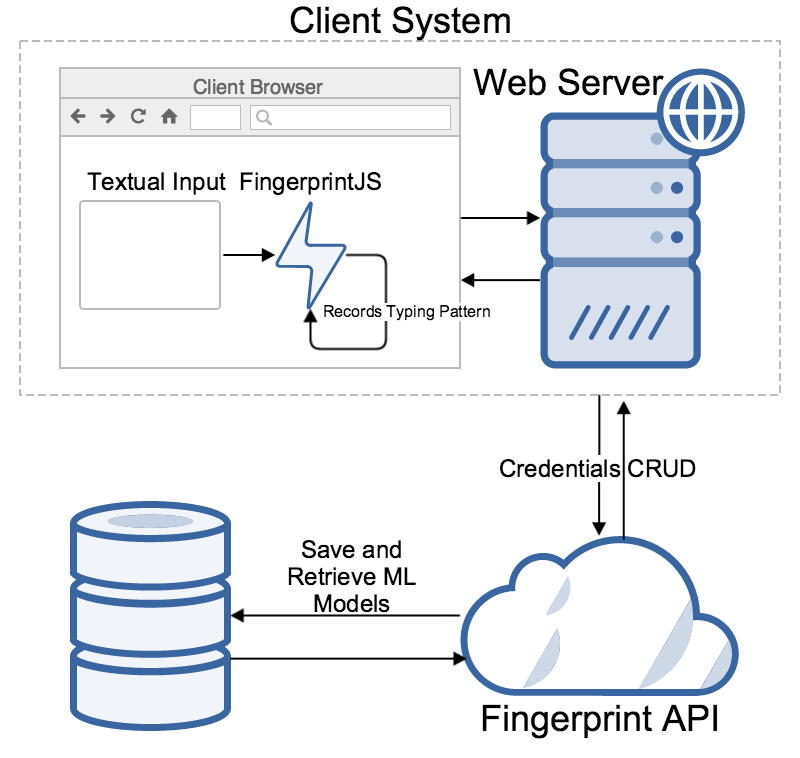
\includegraphics[width=8cm]{SystemDesign.png}}
\end{center}

\section{Modelo conceitual}
\label{modelo}
Aqui entra a modelagem do processo de decisão.

\section{Protótipo}
\label{prototipo}
Aqui entra o nosso POC, sendo feito no GitHub.

\chapter{Experimentos e Resultados}
\label{experimentos}

\chapter{Conclusão}
\label{conclusao}

Excelente trabalho, time!

\end{document}
